\documentclass[letterpaper]{article} % DO NOT CHANGE THIS
\usepackage[submission]{aaai2027} % DO NOT CHANGE THIS
\usepackage[hyphens]{url} % DO NOT CHANGE THIS
\usepackage{graphicx} % DO NOT CHANGE THIS
\urlstyle{rm} % DO NOT CHANGE THIS
\def\UrlFont{\rm} % DO NOT CHANGE THIS
\usepackage{natbib} % DO NOT CHANGE THIS AND DO NOT ADD ANY OPTIONS TO IT
\usepackage{caption} % DO NOT CHANGE THIS AND DO NOT ADD ANY OPTIONS TO IT
\frenchspacing % DO NOT CHANGE THIS

\usepackage{amsmath,amssymb,amsthm}
\theoremstyle{plain}
\newtheorem{theorem}{Theorem}
\newtheorem{proposition}{Proposition}
\usepackage{booktabs}

\pdfinfo{
/TemplateVersion (2027.1)
}

\newcommand{\wcrit}{w_{\mathrm{crit}}}
\newcommand{\PT}{\mathrm{PT}}

\setcounter{secnumdepth}{2}

\title{Supplementary Material:\\Coordination-Collapse Phase Boundary in Policy-Gradient Cooperative MARL}

\author{
  Anonymous Submission
}
\affiliations{
  Paper under double-blind review
}

\begin{document}

\maketitle

\noindent This document contains the apparatus supporting the main paper: full experimental
setup and hyperparameters (\S\ref{sec:s_setup}), the complete loss-aversion sweep and
baseline reconciliation (\S\ref{sec:s_results}), the full mean-field derivation and all three
theorems (\S\ref{sec:s_mechanism}), the cross-environment and cross-algorithm detail
(\S\ref{sec:s_generalization}), both boundary-condition ablations (\S\ref{sec:s_ablations}),
the pre-registered signal-to-noise probe (\S\ref{sec:s_snr}), the exploration-noise ablation
(\S\ref{sec:s_entropy}), threshold robustness (\S\ref{sec:s_robustness}), notation
(\S\ref{sec:s_notation}), and a claim--evidence ledger (\S\ref{sec:s_ledger}). Section,
equation, and figure references to the main paper are by name. All designs were
pre-registered before execution (commit hash withheld for anonymity, released on acceptance).

% =======================================================================
\section{Experimental Setup in Full}
\label{sec:s_setup}

\paragraph{Primary substrate.}
\texttt{NetworkManagement-v1} from or-gym~\citep{hubbs2020orgym}: a six-node multi-echelon
inventory network with Poisson demand ($\mu{=}20$) on the retail edge, 30-period episodes,
uniform lead times. Node~1 (retail-facing) follows a fixed demand-pull policy, stabilizing
the demand signal; nodes~2--6 are trained as cooperative PPO agents. Actions are
parameterized via a base-stock wrapper mapping each agent's continuous action to a target
inventory level $S\in[0,500]$, with order quantity $Q=\max(0,S-\mathrm{IP})$ where
$\mathrm{IP}$ is inventory position. The substrate extends prior DRL inventory work, the
Beer Distribution Game Dec-POMDP of \citet{oroojlooyjadid2022}, the multi-echelon A3C results
of \citet{gijsbrechts2022}, and single-echelon MARL~\citep{marlim2023}, to a six-node
network with per-node agents.

\paragraph{Algorithm and evaluation.}
Each agent runs PPO~\citep{schulman2017ppo} with a shared MLP policy
(\texttt{n\_steps}${=}128$, \texttt{batch\_size}${=}256$), implemented with
Stable-Baselines3~\citep{raffin2021sb3} and PettingZoo/SuperSuit
vectorization~\citep{terry2021pettingzoo,terry2020supersuit}. Evaluation is deterministic
over 10 episodes with 20 seeds per condition.

\paragraph{Experiment inventory.}
Table~\ref{tab:experiments} summarizes the seven primary experiments; total run count 1{,}524.

\begin{table}[t]
\centering
\caption{Primary experiment summary (same environment and algorithm; $\alpha{=}\beta{=}1$ is
the linear no-PT condition).}
\label{tab:experiments}
\small
\setlength{\tabcolsep}{4pt}
\begin{tabular}{llrrrr}
\toprule
Exp & Purpose & $\lambda$ & $\alpha,\beta$ & Seeds & Runs \\
\midrule
A @150k & Struct.\ boundary & 1 & 1,1 & 20 & 220 \\
A @300k & Struct.\ boundary & 1 & 1,1 & 20 & 140 \\
C & Basin control & 1 & 1,1 & 12 & 144 \\
N & Null baseline & 1 & 1,1 & 20 & 180 \\
B-Red. & Behav.\ decomp. & 1,3,7 & 0.88 & 20 & 300 \\
$\lambda$-sweep & Loss-av.\ law & 2,4,5,6 & 0.88 & 20 & 400 \\
T (600k) & Metastability & 1 & 0.88 & 20 & 140 \\
\bottomrule
\end{tabular}
\end{table}

\paragraph{Basin control (rules out initialization).}
Exp~C rules out initialization as a collapse driver. Within-$w$ correlations between
$S_{\mathrm{init}}$ and converged $S$ are $-0.11$ ($w{=}0.5$), $-0.38$ ($w{=}0.85$), and
$-0.36$ ($w{=}1.0$), all near zero and inconsistent with initialization dominating; the
collapsed/survived assignment is insensitive to where agents start.

% =======================================================================
\section{Full Behavioral Sweep and Baseline Reconciliation}
\label{sec:s_results}

\paragraph{The recurring $\wcrit$ values.}
There is one structural null; the other recurring numbers are a horizon measurement of it and
a curvature \emph{result}, not independent baselines (Table~\ref{tab:baselines}).

\begin{table}[t]
\centering
\caption{The recurring $\wcrit$ values and the single role each plays.}
\label{tab:baselines}
\small
\begin{tabular}{lll}
\toprule
$\wcrit$ & Condition & Role \\
\midrule
$0.666$ & $\alpha{=}\beta{=}1$, 300k & canonical null \\
$0.685$ & $\alpha{=}\beta{=}1$, 300k (Exp~N) & null, reproduced \\
$0.822$ & $\alpha{=}\beta{=}1$, 150k & null at shorter horizon \\
$0.586$ & $\alpha{=}\beta{=}0.88$, $\lambda{=}1$ & curvature result \\
\bottomrule
\end{tabular}
\end{table}

\paragraph{Full loss-aversion sweep.}
Table~\ref{tab:lambda_sweep} gives the complete $\lambda{=}1{\dots}7$ sweep with Firth penalized
fits. The increase is monotone up to estimation noise at the high-$\lambda$ plateau:
$\wcrit$ rises strictly from $\lambda{=}1$ to $\lambda{=}5$ then saturates near $0.84$--$0.85$
($\lambda{=}5,6$ statistically indistinguishable). At high loss aversion the transition is
very steep and falls between adjacent grid points (collapse fractions $1.00,1.00,1.00,0.55,
0.00$ at $w\in\{0.5,0.65,0.75,0.85,0.95\}$ for $\lambda{=}7$), so the boundary remains
identifiable (the $w{=}0.85$ cell is interior, $11/20$ collapsed) but the unpenalized MLE
slope diverges. Firth penalized logistic regression is stable here; all seven slopes are
significant ($p<10^{-3}$) and the Firth $\wcrit$ matches the bootstrap to within $0.019$,
confirming the large unpenalized slopes at $\lambda{=}5,7$ were a fitting artifact, not
separation. The high-$\lambda$ plateau is a behavioral saturation, not a $w{=}1$ ceiling
artifact: at $\lambda{=}7$ coordination is fully restored (collapse fraction $0.00$) already
at $w{=}0.95$, consistent with the bounded affine law in which $\wcrit(\lambda)\to1$ only as
$\lambda\to\infty$. The $\lambda{\geq}5$ values in Table~\ref{tab:lambda_sweep} use a finer
$w\in\{0.80,0.90\}$ grid added specifically to resolve the steep transition; this places two
interior points across each high-$\lambda$ boundary and halves the CI widths
($0.038,0.033,0.024$ at $\lambda{=}5,6,7$) relative to the single $w{=}0.85$ cell, giving the
clean monotone $0.825\to0.835\to0.852$.

\begin{table}[t]
\centering
\caption{Full loss-aversion sweep ($\alpha{=}\beta{=}0.88$, 300k, 20 seeds/$(w,\lambda)$
cell, $n{=}100$ runs/$\lambda$). $\wcrit$ with bootstrap 95\% CIs; slope/$p$ from Firth
penalized logistic regression.}
\label{tab:lambda_sweep}
\small
\begin{tabular}{ccccc}
\toprule
$\lambda$ & $\wcrit$ & 95\% CI & Firth $b_1$ & $p$ \\
\midrule
1 & 0.586 & [0.539, 0.624] & $-14.7$ & $1.2\times10^{-6}$ \\
2 & 0.715 & [0.687, 0.745] & $-27.2$ & $4.4\times10^{-6}$ \\
3 & 0.774 & [0.751, 0.798] & $-29.7$ & $5.1\times10^{-6}$ \\
4 & 0.806 & [0.766, 0.841] & $-36.8$ & $5.5\times10^{-6}$ \\
5 & 0.825 & [0.806, 0.844] & $-53.1$ & $4.7\times10^{-4}$ \\
6 & 0.835 & [0.817, 0.850] & $-24.7$ & $2.5\times10^{-6}$ \\
7 & 0.852 & [0.841, 0.864] & $-43.1$ & $1.5\times10^{-3}$ \\
\bottomrule
\end{tabular}
\end{table}

\paragraph{Metastability under matched curvature.}
The 600k row of the main-paper heatmap uses $\alpha{=}\beta{=}0.88$, which shifts $\wcrit$
left by $0.100$, so those collapse fractions are partly curvature-deflated. Under matched
$\alpha{=}\beta{=}1$ (Exp~0b, 20 seeds, 600k), $P(\mathrm{collapse}\mid w{=}0.6)=0.35$ and
$P(\mathrm{collapse}\mid w{=}0.7)=0.20$, versus $0.80$ and $0.40$ at 300k: the horizon slide
holds with curvature held constant; only the figure's 600k magnitude is curvature-inflated.

\paragraph{The metastable slide generalizes.}
The horizon dependence is not a supply-chain artifact. We ran dedicated horizon sweeps under
centralized-critic MAPPO on both transfer environments. On MPE Cooperative Navigation,
$\wcrit$ falls $0.82\to0.68$ as the horizon grows $2\mathrm{M}\to8\mathrm{M}$ env steps (slide
$+0.14$); on Level-Based Foraging it falls $0.33\to0.20$ over $1\mathrm{M}\to4\mathrm{M}$
(slide $+0.13$), each with non-overlapping bootstrap intervals at the endpoints. Both match
the supply-chain direction (boundary slides left with more training), so the metastability
result (like the loss-aversion direction) holds across environments and algorithms, not just
on the primary substrate.

\paragraph{The four-horizon log-linear fit.}
On the supply chain we measured $\wcrit$ at four matched risk-neutral horizons
(Table~\ref{tab:horizons}). The four points fall on a log-linear law $\wcrit=2.44-0.138\ln T$
(RMSE $0.027$), the Kramers escape-time prediction that $\wcrit$ falls as $-\ln T$ toward the
deterministic floor $\wcrit^0=c/(c+g)$. The two longer horizons (450k, 900k) have bootstrap CIs of
width ${\le}0.04$, so the law is a fitted four-point relationship, not a two-point extrapolation.

\begin{table}[t]
\centering \small
\caption{Matched risk-neutral horizons ($\alpha{=}\beta{=}1$, $\lambda{=}1$). $\wcrit$ with
bootstrap 95\% CIs; the four points fit $\wcrit=2.44-0.138\ln T$ at RMSE $0.027$.}
\label{tab:horizons}
\begin{tabular}{lcc}
\toprule
$T$ (env steps) & $\wcrit$ & 95\% CI \\
\midrule
150k & 0.822 & [0.785, 0.858] \\
300k & 0.666 & [0.635, 0.694] \\
450k & 0.622 & [0.603, 0.641] \\
900k & 0.573 & [0.547, 0.598] \\
\bottomrule
\end{tabular}
\end{table}

\medskip\noindent The derived affine law~\eqref{eq:wcrit_lambda} and its out-of-sample fit
(RMSE $0.014$ across all seven points) are shown and discussed in the main paper; the
derivation of its form is given in \S\ref{sec:s_mechanism} below.

% =======================================================================
\section{Mean-Field Mechanism in Full}
\label{sec:s_mechanism}

This section develops the mechanism the main paper summarizes. It is a mechanistic account of
why the boundary exists and how it moves, not a closed-form derivation of $\wcrit$. We are
explicit about what is derived, what is calibrated, and what is not claimed (Table~\ref{tab:ledger_full}).
As noted in the main paper, the deep-MARL contribution is the learning-dynamics analogue of
the established EGT result~\citep{mengesha2025}: here the driver is the signal-to-noise ratio
of the policy gradient under exploration, not selection pressure over fixed strategies.

\subsection{Gradient flow and its noise}
Each agent $i$ runs PPO on a Gaussian policy over its normalized base-stock action
$a_i\in[0,1]$ with mean $\mu_i$ and exploration scale $\sigma$. The shaped reward is the
centralization blend through the CPT value function $v$,
\begin{equation}
 r_i = v\!\big((1-w)\,\ell_i(a_i,a_{-i}) + w\,G(a)\big),\quad G(a)=\textstyle\sum_j \ell_j,
 \label{eq:blend}
\end{equation}
with $\ell_i$ node $i$'s local profit and $G$ system profit. For a Gaussian policy the PPO
mean update is a stochastic estimate of the return gradient, so the mean follows a mean-field
Langevin (Fokker--Planck) equation
\begin{equation}
 \mathrm{d}\mu_i = \underbrace{\eta\,\partial_{\mu_i}\mathbb{E}[(1{-}w)\ell_i + wG]}_{\text{drift } D(w)}\,\mathrm{d}t
 + \sqrt{2\,\Theta(w)}\;\mathrm{d}W .
 \label{eq:langevin}
\end{equation}
Because each partner's local profit is blended into the global term, partner exploration
$\sigma$ enters agent $i$'s gradient estimate through the global channel, so the diffusion
carries a centralization-weighted cross-agent piece
\begin{equation}
 \Theta(w)\propto\tfrac{\sigma^2}{B}\big[(1{-}w)^2 s_\ell^2 + w^2(N{-}1)\kappa^2\big],
 \label{eq:diffusion}
\end{equation}
with batch size $B$, local sensitivity $s_\ell$, cross-agent sensitivity $\kappa$; the diffusion
$\Theta$ carries the centralization and exploration dependence, not the behavioral one. Loss
aversion instead acts on the \emph{drift}: by asymmetrically down-weighting gains against losses,
the CPT transform biases the expected update toward the conservative lazy action, i.e.\
$\partial_\lambda F<0$, weakening the cooperative drift $D$ and so the SNR. A finite-difference
probe confirms this loss-domain gradient asymmetry (\S\ref{sec:s_mechanism}).

\subsection{The boundary is a signal-to-noise crossing}
A direct finite-difference probe of $\ell_i$ and $G$ along the base-stock axis confirms the
asymmetry the model needs: an upstream node's inventory is a \emph{local cost} (holding and
procurement reduce its profit) but a \emph{global benefit} (it averts downstream stockouts).
Writing the linearized marginals $\partial_a\mathbb{E}\ell\to-c$, $\partial_a\mathbb{E}G\to+g$
($c,g>0$), the cooperative drift is
\begin{equation}
 D(w)=\eta\big[wg-(1-w)c\big].
 \label{eq:drift}
\end{equation}
Escape from the lazy basin requires $\mathrm{SNR}(w)=D(w)/\sqrt{\Theta(w)}\gtrsim\kappa_c$
for an $\mathcal{O}(1)$ critical $\kappa_c$ set by the training budget; the crossing defines
$\wcrit$. In the low-noise limit $\Theta\to0$ this reduces to $D(w)=0$, i.e.
$\wcrit^0=c/(c+g)$, the asymptotic ($T\to\infty$) boundary; finite exploration noise raises
the operative boundary above it. The coefficients $c,g,\sigma,\kappa_c$ are not derived in
closed form from the multi-echelon cost matrix; the model is calibrated and its content is the
functional predictions, not the magnitude.

\subsection{Sharpness and metastability}
Escape is a Kramers first-passage problem, $\tau\sim\tau_0\exp(\Delta U/\Theta)$,
exponentially sensitive to $\mathrm{SNR}$, so collapse probability switches abruptly across
$\wcrit$ (matching the steep logistic fits). Collapse at finite horizon means $\tau>T$; as
$T$ grows a smaller $\mathrm{SNR}$ (hence smaller $w$) suffices, so $\wcrit(T)$ decreases
monotonically toward $\wcrit^0$, the observed $0.822\to0.666$ slide, following the
$\propto-\ln T$ Kramers trend.

\subsection{Formal account: predicted versus calibrated}
Let $x\in[0,1]$ be a macroscopic order parameter (fraction of agents coordinating) evolving as
\begin{equation}
 \mathrm{d}x_t = F(x_t,w,\lambda)\,\mathrm{d}t + \sqrt{\Sigma(x_t,N)}\,\mathrm{d}W_t,
 \label{eq:sde}
\end{equation}
with $F$ the mean-field drift (so $\partial_w F>0$ and $\partial_\lambda F<0$ follow from the
payoff structure: $w$ weights the cooperation gradient $+g$, $\lambda$ scales only the loss
domain) and $\Sigma>0$ the gradient-noise variance. $x$ is \emph{latent}: consistent with our
pre-registered probe (\S\ref{sec:s_snr}) it is not recoverable from policy statistics, so the
claims concern its law, not a measured trajectory.

\begin{theorem}[Mean-field criticality, $N\to\infty$]\label{thm:mf}
If $\Sigma(x,N)=D(x)/N$, then as $N\to\infty$ the dynamics become deterministic,
$\dot x=F(x,w,\lambda)$, and the coordinating basin disappears via a saddle-node bifurcation.
The mean-field threshold $\wcrit^{\mathrm{MF}}$ is the unique solution of
$F(x^\ast,w,\lambda)=0$, $\partial_x F(x^\ast,w,\lambda)=0$, a closed-form function of the
payoff and prospect-theory parameters.
\end{theorem}
\begin{proof}
With $\Sigma=D(x)/N\to0$ the noise in \eqref{eq:sde} vanishes and the flow is $\dot x=F$. A
coordinating stable node and an unstable saddle bound the basin; the basin vanishes when they
collide, i.e.\ $F=0$ and $\partial_x F=0$ coincide (saddle-node). As $F$ is closed-form in the
payoff and CPT functions, so is its root $\wcrit^{\mathrm{MF}}$.
\end{proof}

\begin{theorem}[Calibration gap, finite $N$ and horizon $T$]\label{thm:gap}
For finite $N$ with correlated CTDE updates, $\Sigma(x,N)>0$, and collapse is a noise-induced
escape rather than a bifurcation. The empirical boundary is the metastability root
$\tau(w,\lambda)=T$ of the Kramers mean first-passage time
\begin{equation}
 \tau\asymp\exp(\Delta U),\quad
 \Delta U=\int_{x^\ast_{\mathrm{lazy}}}^{x^\ast_{\mathrm{saddle}}}\frac{-2F(z,w,\lambda)}{\Sigma(z,N)}\,\mathrm{d}z,
 \label{eq:barrier}
\end{equation}
and $\wcrit^{\mathrm{Emp}}\neq\wcrit^{\mathrm{MF}}$ in general; the offset cannot be isolated
without measuring $\Sigma$.
\end{theorem}
\begin{proof}
The stationary density of \eqref{eq:sde} is $P_{ss}(x)\propto\exp[-U_{\mathrm{eff}}(x)]$ with
$U_{\mathrm{eff}}(x)=-\int_0^x 2F/\Sigma\,\mathrm{d}z$, giving the barrier $\Delta U$ of
\eqref{eq:barrier}; Kramers' rate yields $\tau\asymp e^{\Delta U}$. At finite $T$, collapse is
failure to escape the lazy basin within budget ($\tau>T$), so the boundary solves
$\tau(w,\lambda)=T$. Since $\Sigma$ is the
intractable covariance of PPO updates, $\Delta U$ and hence $\wcrit^{\mathrm{Emp}}$ require
calibration. The two notions coincide as limits: at finite $(N,T)$ escaping the lazy basin needs a
$w$ above the deterministic floor, and $\wcrit^{\mathrm{Emp}}(T)\downarrow\wcrit^{\mathrm{MF}}$ as
$T\to\infty$.
\end{proof}

\begin{proposition}[Sign propagation of the loss-aversion shift]\label{thm:sign}
Assume $\Sigma>0$ and the payoff premise $\partial_\lambda F(x,w,\lambda)<0$ for all
$x\in[x^\ast_{\mathrm{lazy}},x^\ast_{\mathrm{saddle}}]$ (verified by finite-difference probe;
\S\ref{sec:s_mechanism}). Then $\partial_\lambda \wcrit^{\mathrm{Emp}}>0$.
\end{proposition}
\begin{proof}
The escape barrier of \eqref{eq:barrier} is $\Delta U=\int_{x^\ast_{\mathrm{lazy}}}^{x^\ast_{\mathrm{saddle}}}(-2F/\Sigma)\,\mathrm{d}z$. The
integration limits depend on $\lambda$, but the Leibniz boundary terms vanish because $F=0$ at both
fixed points (to leading order in the noise the endpoints are the deterministic zeros of
$F$), so only the integrand varies:
$\partial_\lambda\Delta U=\int(-2\,\partial_\lambda F/\Sigma)\,\mathrm{d}z>0$ pointwise, since
$\Sigma>0$ and $\partial_\lambda F<0$ on the whole interval, independent of the sign of $F$.
Here $\tau$ is the mean time to escape the lazy basin and reach coordination, with collapse at
finite horizon being $\tau>T$: a \emph{higher} barrier \emph{lengthens} escape
($\partial_\lambda\tau>0$), while raising $w$ steepens the cooperative drift ($\partial_w F>0$),
lowers the barrier, and shortens escape ($\partial_w\tau<0$).
The implicit function theorem on $\tau(w,\lambda)-T=0$ gives
$\mathrm{d}\wcrit^{\mathrm{Emp}}/\mathrm{d}\lambda=-\partial_\lambda\tau/\partial_w\tau>0$.
The magnitude depends on $\Sigma$ (Theorem~\ref{thm:gap}), but the direction is guaranteed by the
drift alone. The identical argument with $\partial F$ signs reversed for concave--convex
curvature gives the opposite shift.
\end{proof}

\subsection{Opposite signs and the derived affine law}
Concave--convex curvature ($\alpha,\beta<1$) compresses gains and losses \emph{symmetrically},
lowering the variance entering $\Theta$, raising the SNR, and \emph{lowering} $\wcrit$; loss
aversion ($\lambda>1$) acts \emph{asymmetrically} on the downside, biasing the drift toward the
conservative action ($\partial_\lambda F<0$), lowering the SNR, and \emph{raising}
$\wcrit$. The signs are fixed before any data. The functional form follows by splitting the
marginal mass into gain/loss domains; only the loss domain scales with $\lambda$, giving
\begin{equation}
 \wcrit(\lambda)=\frac{\phi(\lambda)}{\phi(\lambda)+\gamma},\quad\phi(\lambda)=1+\rho(\lambda-1),
 \label{eq:wcrit_lambda}
\end{equation}
with $\rho\in[0,1]$ bounded by the theory. The ratio $\gamma$ is the \emph{effective}
gain-to-loss marginal-mass ratio at the fixed finite horizon; it is not the drift floor
$c/(c+g)$ of \eqref{eq:drift} (numerically $\gamma\approx0.71$ versus $c/(c+g)\approx0.44$ from the
horizon extrapolation), the two coinciding only as $T\to\infty$, where the boundary reaches the
drift zero, which loss aversion (scaling the drift, not its zero) leaves fixed. Fixing $\gamma$ from the
$\lambda{=}1$ baseline and $\rho=0.61$ from three calibration points ($\lambda\in\{1,3,7\}$), held
fixed and tested out of sample against $\lambda\in\{2,4,5,6\}$, gives
$\wcrit^{\text{pred}}=\{0.586,0.695,0.759,0.800,0.830,0.851,0.868\}$ versus
$\wcrit^{\text{meas}}=\{0.586,0.715,0.774,0.806,0.825,0.835,0.852\}$, RMSE $0.014$ (plotted in
the main paper). The one systematic residual is mild concave overshoot at the plateau,
consistent with agents endogenously reducing loss exposure as $\lambda$ grows.

\begin{table}[t]
\centering
\caption{What the mean-field mechanism claims (extended version of the main-paper ledger,
adding the exploration-noise row and the MPE-null detail).}
\label{tab:ledger_full}
\small
\begin{tabular}{p{0.27\linewidth}p{0.63\linewidth}}
\toprule
\textbf{Derived (no fit)} & opposite signs of curvature vs.\ loss aversion; monotone
$\wcrit(\lambda)$; affine $\phi(\lambda)$ with $\rho\in[0,1]$; phase-transition sharpness;
$\wcrit$ decreasing with $T$; $\wcrit$ increasing with exploration noise. \\
\midrule
\textbf{Empirically confirmed} & opposite signs and affine form; horizon slide (also on MPE,
LBF); exploration-noise dependence (supply chain and LBF; predicted null on MPE). \\
\midrule
\textbf{Calibrated} & effective ratio $\gamma$; loss-domain share $\rho$; noise scale setting absolute $\wcrit$. \\
\midrule
\textbf{Not claimed} & closed-form $\wcrit$ from the cost matrix; numerical magnitude on any
axis; the mild concavity beyond leading order. \\
\bottomrule
\end{tabular}
\end{table}

% =======================================================================
\section{Generalization Detail}
\label{sec:s_generalization}

\subsection{Cross-environment: MPE Cooperative Navigation}
Three agents cover three landmarks in a continuous 2-D arena (discrete actions, 50-step
episodes). The locally rational action under the herding incentive is to stay near
teammates, collectively disastrous, as agents cluster and no landmark is covered. We set
\texttt{local\_ratio}${=}0$ so the raw reward is the pure global team score; the herding term
is defined by our wrapper. Collapse is per-step landmark occupancy (fraction of landmarks
within a fixed radius of some agent), a behavioral metric invariant to reward scale and so
unaffected by the CPT transform. Unlike the supply chain (per-agent incentives), MPE's
coordination reward is shared-global, which under independent learners confounds behavioral
collapse with credit-assignment failure; we therefore train MPE with centralized-critic
MAPPO~\citep{yu2022surprising,lowe2017multi}. We set the herding scale so the null boundary
is interior ($\wcrit{=}0.74$) and ran the full $\lambda$-sweep (1{,}760 runs, 20 seeds/cell;
Figure~\ref{fig:mpe_lambda_curves}). The loss-aversion effect replicates, $\wcrit$ rises
$0.78\to0.89$ over $\lambda{=}1\to7$, rising in envelope but non-monotone at intermediate
$\lambda$, excess $+0.158$ $[0.108,0.212]$ at $\lambda{=}7$ and $+0.101$ $[0.055,0.150]$ at
$\lambda{=}3$ (matching the supply chain's $+0.089$). The curvature effect does \emph{not}
replicate ($+0.042$ $[-0.009,0.092]$, opposite in sign), and the affine form fits MPE only to
RMSE $0.05$.

\begin{figure}[t]
 \centering
 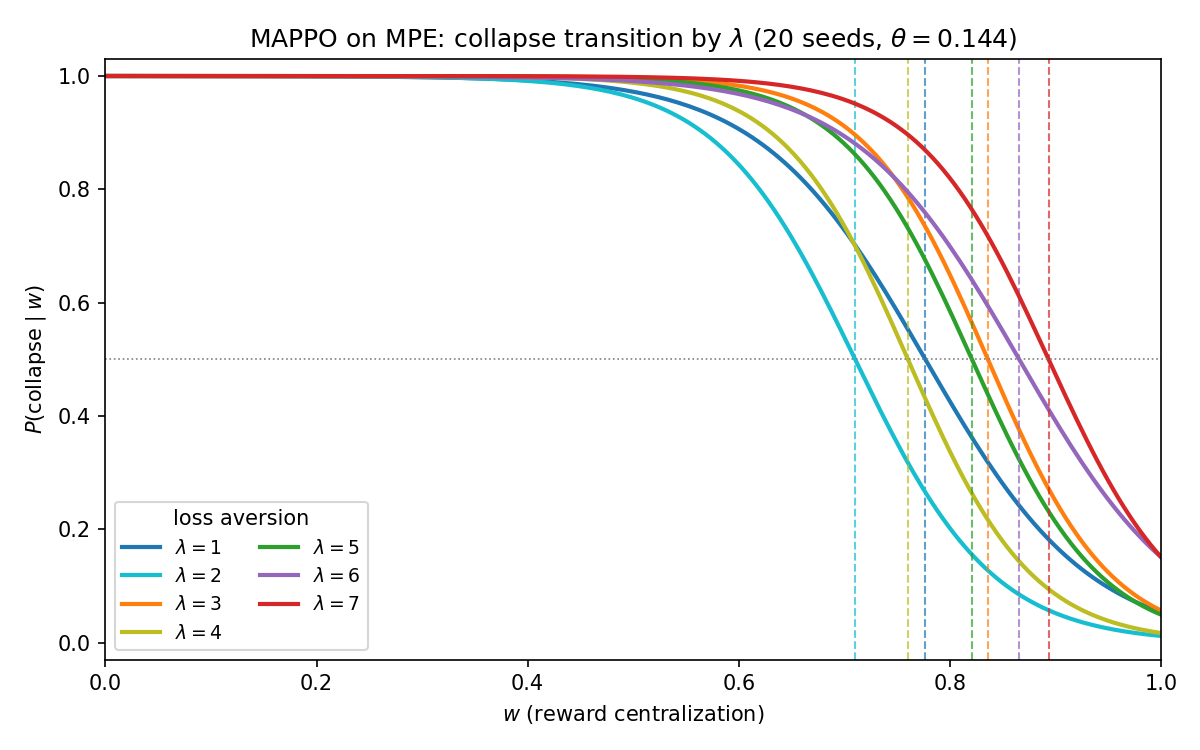
\includegraphics[width=0.9\columnwidth]{Figures/mappo_mpe_lambda_curves}
 \caption{MAPPO on MPE Cooperative Navigation: fitted $P(\mathrm{collapse}\mid w)$ for
  $\lambda{=}1,\dots,7$ ($\alpha{=}\beta{=}0.88$, centralized critic, collapse = landmark
  occupancy below $\theta{=}0.144$). The family shifts rightward with $\lambda$, the same
  loss-aversion signature, under a different environment and algorithm.}
 \label{fig:mpe_lambda_curves}
\end{figure}

\subsection{A third environment: Level-Based Foraging}
LBF~\citep{christianos2020shared} has a public-goods incentive: agents pay an effort cost to
load food cooperatively, so the locally rational action is to free-ride. Natively discrete,
unrelated to logistics or navigation, trained under centralized-critic MAPPO (matching MPE so
only the environment varies), full $\lambda$-sweep, same collapse-midpoint criterion (1{,}600
runs). The risk-neutral null is low and tight ($\wcrit\approx0.08$); curvature moves it
\emph{right} by $+0.18$ (opposite to the supply chain). Loss aversion drives $\wcrit$ from
$0.26$ at $\lambda{=}1$ to $0.83$ at $\lambda{=}4$, monotone with non-overlapping endpoint CIs
(the pre-registered criterion), robust to the collapse threshold. For $\lambda\geq5$ the
boundary saturates against the centralization ceiling: the logistic $\wcrit$ extrapolates to
$w\geq1$ (outside the measured $w\in[0,0.95]$ grid), so these points are \emph{not} interior
estimates and we label them exploratory in the precise sense that their $\wcrit$ lies beyond the
range any run samples, their location is bounded below by $0.95$ but not upper-bounded by the data.
An added intermediate level $w{=}0.90$ tightens the mid-$\lambda$ estimates and confirms the
saturation, but does not bring the $\lambda\geq5$ crossings inside the grid. The supply chain's affine law does not transfer: with $\gamma$ fixed
from $\lambda{=}1$, the best-fit slope saturates at its bound and misfits LBF by RMSE $0.15$,
converting the form's substrate-specificity from assertion to measured result.

\subsection{Cross-algorithm: MAPPO on the supply chain}
To isolate the algorithm from the environment, we re-run the full sweep on the \emph{identical}
substrate, grid, seeds, label, and hyperparameters, changing only the learner from independent
PPO to centralized-critic MAPPO (700 runs; Figure~\ref{fig:mappo_curves}). $\wcrit$ rises
$0.796\,[0.742,0.860]$ at $\lambda{=}1$ to $0.889\,[0.856,0.917]$ at $\lambda{=}7$, monotone
from $\lambda{=}2$ ($0.747,0.795,0.800,0.851,0.861,0.889$), endpoint CIs non-overlapping. The
direction generalizes while the absolute level does not: MAPPO sits above PPO at low $\lambda$
(most visibly $\lambda{=}1$, $0.796$ vs $0.586$, where MAPPO's transition is shallow and the
estimate noisier), converging by $\lambda\geq4$ ($|\Delta\wcrit|\leq0.04$).

\begin{figure}[t]
 \centering
 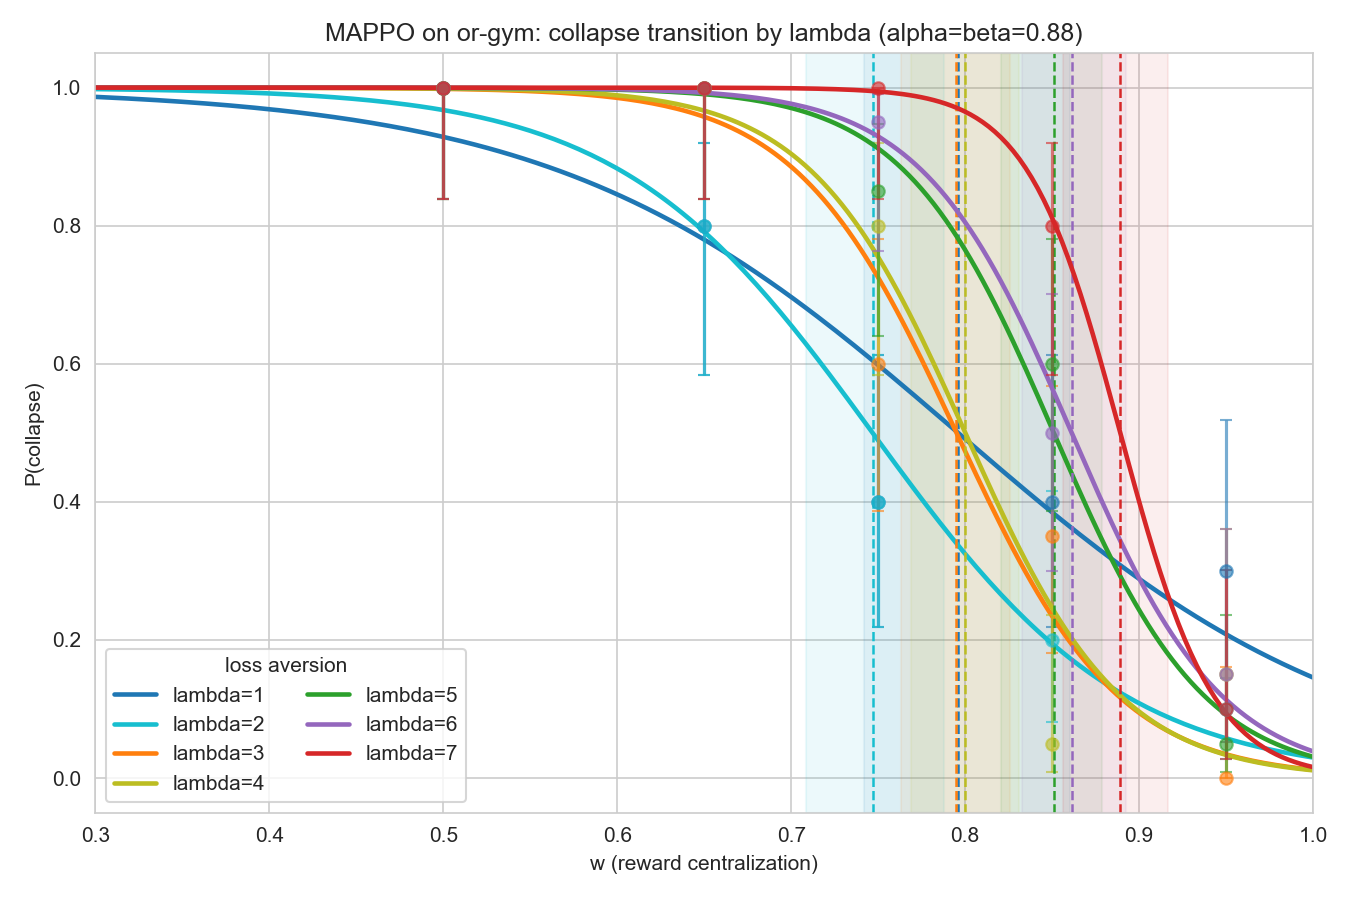
\includegraphics[width=0.9\columnwidth]{Figures/mappo_orgym_collapse_curves}
 \caption{Centralized-critic MAPPO on the supply chain: $P(\mathrm{collapse}\mid w)$ for
  $\lambda{=}1,\dots,7$ (700 runs). As under PPO, the family shifts rightward with loss
  aversion, confirming the effect is not an artifact of independent PPO.}
 \label{fig:mappo_curves}
\end{figure}

% =======================================================================
\section{Two Boundary-Condition Ablations}
\label{sec:s_ablations}

\subsection{Action representation}
The mechanism predicts that destroying the continuous policy gradient removes the boundary.
Value-based learners need discrete actions, so we discretized the base-stock control into
$K{=}11$ bins and ran IQL and QMIX on the identical reward pipeline, $w$-grid, and label; both
produced a flat, $w$-independent collapse rate with no fittable $\wcrit$. To isolate the
cause, a single-variable control (PPO on the same $K{=}11$ discrete shell) also goes flat
(Table~\ref{tab:ablation_action}). Discretization \emph{alone} erases the boundary, so the
value-based nulls need no appeal to the learning paradigm. This is not a claim that
discreteness per se removes the boundary: MPE is natively discrete and retains it. Coarse bins
snap the policy to a stable interior level and never visit the near-threshold $(s,S)$ region
where collapse occurs, exactly the continuous-gradient prediction. The effect is a
coarse-discretization boundary condition, substrate-specific like the curvature sign, and a
confirmed prediction, not a negative result.

\begin{table}[t]
\centering \small
\caption{Action-representation ablation. The control (last row) changes only the action space
while holding the learner at PPO, isolating coarse discretization, not the value-based
paradigm, as what erases the boundary.}
\label{tab:ablation_action}
\begin{tabular}{lll}
\toprule
Learner & Action space & Boundary? \\
\midrule
PPO / MAPPO & continuous & yes \\
QMIX (centralized value) & discrete $K{=}11$ & no \\
IQL (independent value) & discrete $K{=}11$ & no \\
PPO (control) & discrete $K{=}11$ & \textbf{no} \\
\bottomrule
\end{tabular}
\end{table}

\subsection{Credit assignment}
The boundary is measurable only with a learner that can coordinate on a shared-reward task.
On MPE, independent PPO never reaches the coordinated regime at \emph{any} $w$ (collapse
fraction $1.0$ throughout, including maximal centralization; Figure~\ref{fig:mpe_floor}), so
behavioral collapse cannot be distinguished from inability to assign credit. Centralized-critic
MAPPO recovers coordination (collapse fraction falls to $0.35$, occupancy crosses the threshold
near $w\approx0.6$). The same floor appears on LBF. The boundary is therefore measurable only
with a centralized critic on shared-reward tasks, why we match one to such environments: a
necessity, not a convenience.

\begin{figure}[t]
 \centering
 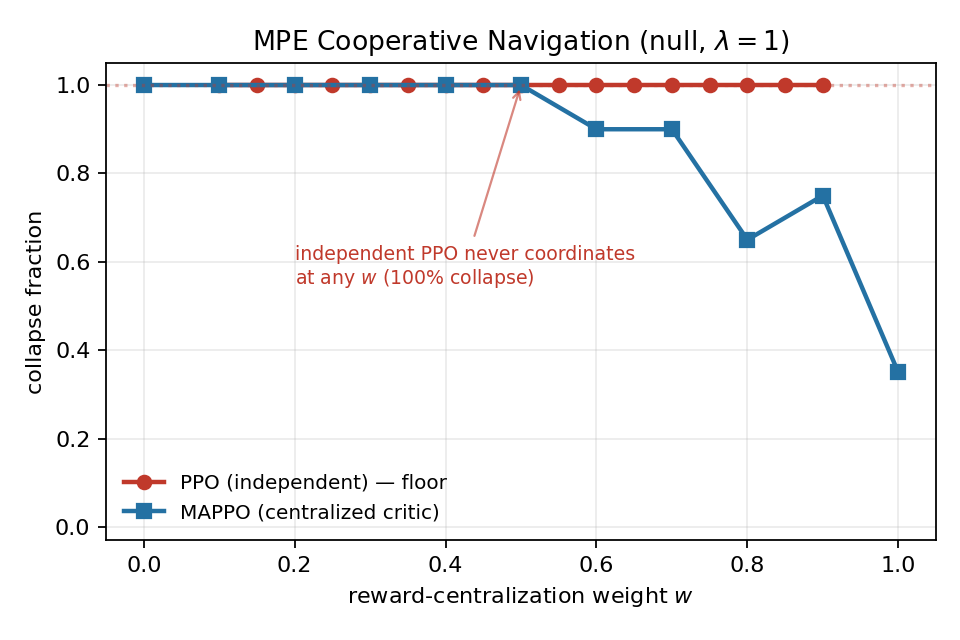
\includegraphics[width=0.9\columnwidth]{Figures/mpe_ppo_coordination_floor}
 \caption{Credit-assignment ablation on MPE (null, $\lambda{=}1$). Independent PPO collapses
  at every $w$ (a coordination floor), while centralized-critic MAPPO crosses the boundary.
  The behavioral boundary is exposed only once credit assignment is handled.}
 \label{fig:mpe_floor}
\end{figure}

% =======================================================================
\section{Pre-registered Signal-to-Noise Probe}
\label{sec:s_snr}

The mean-field account calibrates the magnitude of $\wcrit$ rather than predicting it, because
the drift and diffusion coefficients are properties of the stochastic learning dynamics. We
pre-registered a direct measurement to upgrade magnitude from calibrated to predicted, fixing
its analysis before running. \textbf{Observable:} during PPO training we log the mean
base-stock action $\mu$ once per update and, over a fixed early window, estimate drift $D(w)$
(mean increment) and diffusion $\Theta(w)$ (increment variance/2), forming
$\mathrm{SNR}(w)=D(w)/\sqrt{2\Theta(w)}$. \textbf{Decision rule:} sweep
$w\in\{0.50,\dots,0.90\}$ at the structural condition, 20 seeds/$w$, 150k steps; the mechanism
is corroborated iff the measured crossing's bootstrap 95\% CI contains the matched-horizon
boundary $\wcrit=0.822$. \textbf{Outcome (reported in full):} the collapse-fraction of this
independent sweep crosses $0.5$ at $w=0.82$, reproducing the matched-horizon boundary almost
exactly, a positive robustness check on the boundary. The \emph{drift-sign} observable,
however, was \emph{inconclusive}: the restoring drift in the contested band is weakly positive
across all $w$ with no genuine zero-crossing, so it does not localize $\wcrit$. The reason is
basin geometry, PPO initializes above the cooperative optimum ($S{\approx}250$ vs
$S{\approx}150$), and collapses plunge through the contested band too quickly to sample,
biasing the conditioned drift toward survivors.

\textbf{Non-survivor-biased re-probe (also negative).} We tested the natural fix directly. We
re-ran the identical sweep with the policy re-initialized at the cooperative optimum
($S{\approx}150$, actor mean biased to $a_0{=}{-}0.4$) so that both surviving and collapsing runs
are sampled inside the contested band during early training, and added a second,
initialization-robust \emph{basin-flow} localizer (net early displacement of the policy mean from
the optimum) alongside the restoring-drift statistic. The re-initialization de-biased the
observable (the drift is now smooth and monotone in $w$ rather than flat and noisy) and the
collapse-fraction crossing again reproduced the boundary ($\wcrit\approx0.83$). But neither
statistic \emph{localizes} $\wcrit$: the drift and basin-flow are monotone in $w$ without a
zero-crossing, and their steepest change falls near $w{\approx}0.6$, not at the boundary. The
observable therefore tracks \emph{where the policy sits} rather than \emph{where the boundary is},
which the initialization change does not fix. We consequently report magnitude localization as
genuinely open: the mechanism's sign-level and functional-form predictions stand, but a
magnitude-level prediction of $\wcrit$ remains future work. The re-probe driver and analysis are
released with the code.

% =======================================================================
\section{Exploration-Noise Ablation}
\label{sec:s_entropy}

The mechanism predicts $\wcrit$ rises with exploration noise. Sweeping the PPO entropy
coefficient at the structural condition (300k, 20 seeds, $w\in\{0.5,\dots,0.9\}$), the boundary
rises monotonically: $\wcrit=0.685$ at $\text{ent}{=}0$ (reproducing the null), $0.690$ at
$0.001$, $0.715$ at $0.01$, and beyond $0.05$ the system collapses at every tested $w$
(Table~\ref{tab:entropy}). \textbf{A binding-noise dissociation.} Repeating under MAPPO on the
transfer substrates: on LBF the prediction replicates ($\wcrit$ rises $0.13\to0.37$ over
$\text{ent}\in\{0,0.05\}$, shift $+0.24$, non-overlapping endpoints); on MPE the boundary does
\emph{not} move (shift $+0.05$, overlapping CIs; pooled slope over 1{,}320 runs positive but
not significant, $\beta{=}{+}0.47$, CI $[-3.4,+4.3]$). This is a dissociation predicted by the
mechanism: exploration noise moves the boundary only when it is the binding term in the SNR.
The supply chain and LBF have sparse, sharp landscapes where injected entropy dominates; MPE's
dense distance-shaped reward carries high intrinsic exploration that swamps the added term. The
effect appears exactly where the mechanism says it should and is absent where it says it should
be, a sharper test than uniform replication.

\begin{table}[t]
\centering \small
\caption{Entropy-coefficient ablation ($\alpha{=}\beta{=}1$, $\lambda{=}1$, 300k, 20
seeds/cell). $\wcrit$ with bootstrap 95\% CIs.}
\label{tab:entropy}
\begin{tabular}{cc}
\toprule
entropy coef. & $\wcrit$ (95\% CI) \\
\midrule
0.000 & 0.685 [0.656, 0.710] \\
0.001 & 0.690 [0.667, 0.715] \\
0.010 & 0.715 [0.689, 0.743] \\
0.050 & $>1$ (collapse at all $w$) \\
\bottomrule
\end{tabular}
\end{table}

% =======================================================================
\section{Threshold Robustness}
\label{sec:s_robustness}

We re-estimate $\wcrit$ on Exp~A @300k under nine variants of the collapse definition, varying
the $\bar S$ threshold over $\{8,10,12\}$ and the $\bar\pi$ threshold over
$\{-102.5,-127.1,-152.5\}$. Three variants with $\bar\pi\le-152.5$ are degenerate (the minimum
profit in the dataset is $-128.1$) and excluded. Across the remaining six estimable variants
the maximum deviation from the baseline $\wcrit=0.666$ is $0.015$, well below the CI width: the
collapse definition is robust to $\pm20\%$ threshold perturbation.

% =======================================================================
\section{Notation and Abbreviations}
\label{sec:s_notation}

\begin{table}[h]
\centering \small
\begin{tabular}{lp{0.62\linewidth}}
\toprule
Symbol & Meaning \\
\midrule
$w$ & reward centralization weight, $\in[0,1]$ \\
$\wcrit$ & critical $w$ where $P(\mathrm{collapse}){=}0.5$ \\
$\lambda$ & loss-aversion coefficient ($\lambda{>}1$) \\
$\alpha,\beta$ & CPT value-function curvature (gain/loss) \\
$\rho$ & loss-domain share of marginal incentive, $\in[0,1]$ \\
$g,c$ & marginal global benefit / local cost of cooperation \\
$D(w),\Theta(w)$ & Langevin drift / diffusion of the policy mean \\
$\mathrm{SNR}(w)$ & $D(w)/\sqrt{\Theta(w)}$, escape signal-to-noise ratio \\
$\sigma,\eta,B$ & exploration scale / learning rate / batch size \\
$\Delta U,\tau$ & escape barrier / Kramers first-passage time \\
$T$ & training horizon (environment steps) \\
$\bar S,\bar\pi$ & mean base-stock / mean profit (collapse label) \\
\bottomrule
\end{tabular}
\end{table}

\noindent\textbf{Abbreviations.} MARL (multi-agent reinforcement learning); CTDE (centralized
training, decentralized execution); CPT (cumulative prospect theory); PPO (proximal policy
optimization); MAPPO (multi-agent PPO with a centralized critic); MPE (multi-agent particle
environments); LBF (Level-Based Foraging); SNR (signal-to-noise ratio); CI (confidence
interval).

% =======================================================================
\section{Claim--Evidence Ledger}
\label{sec:s_ledger}

Table~\ref{tab:claim_ledger} states how broadly each headline claim is supported. The loss-aversion
direction is the generalizing core (three environments, two algorithms); the curvature sign and
the downstream-minority cascade are supply-chain-specific, the latter framed as a falsifiable
prediction for directed-flow domains.

\begin{table}[h]
\centering \small
\caption{Each headline claim and the breadth of evidence behind it. Environments: SC (supply
chain), MPE, LBF. Algorithms: PPO, MAPPO.}
\label{tab:claim_ledger}
\begin{tabular}{p{0.46\linewidth}p{0.26\linewidth}p{0.14\linewidth}}
\toprule
Claim & Envs & Algos \\
\midrule
Sharp collapse boundary $\wcrit$ exists & SC, MPE, LBF & PPO, MAPPO \\
Metastability ($\wcrit$ slides with $T$) & SC, MPE, LBF & PPO, MAPPO \\
Loss aversion \emph{raises} $\wcrit$ (dir.) & SC, MPE, LBF & PPO, MAPPO \\
Affine $\lambda$-law (form) & SC & PPO \\
Mechanism fixes sign a priori & SC, entropy abl. & PPO \\
Curvature \emph{lowers} $\wcrit$ (sign) & SC (opp.\ on LBF) & PPO \\
Downstream-minority cascade & SC only & PPO \\
\bottomrule
\end{tabular}
\end{table}

% =======================================================================
\bibliography{references}

\end{document}
